\section{Encaminamiento determinista y adaptativo}\label{sec:p03intro}\pagenumbering{arabic}

\subsection{Objetivo}\label{ssec:p03objetivo}

\normalsize Comprobar y entender el funcionamiento de algoritmos de encaminamiento deterministas y
adaptativos.

\subsection{Desarrollo}\label{ssec:p03desarrollo}

\normalsize La práctica consiste en resolver una serie de  cuestiones relacionadas con el mecanismo de encaminamiento en redes de interconexión. Para realizar esta práctica se hará uso del simulador \emph{SimuRed}, descrito en el apéndice A.

\begin{itemize}
    \item [\textbf{a)}] \textbf{Reproduce una situación con la que se pueda observar el beneficio introducido por el encaminamiento adaptativo en lo que se refiere a nivel de  prestaciones de la red, comparándolo con el caso de encaminamiento determinista.}

    \textbf{Se trata de realizar una pequeña traza para alcanzar el objetivo, y observar mediante una simulación interactiva la evolución de los paquetes por la red.  Utilizar para ello el algoritmo de encaminamiento determinista y el totalmente adaptativo.}

    Para comprobar el beneficio del encaminamiento adaptativo frente al determinista es necesario crear una situación de congestión en la que varios paquetes hagan uso de los mismos recursos. De esta manera, se creará un cuello de botella en ese punto que el encaminamiento adaptativo será capaz de solventar y el determinista no. En este caso, se va a usar la traza mostrada en el Listing \ref{lst:traza3a}.

    \begin{mycode}[style=mycodestyle, caption={Traza para provocar congestión.}, label=lst:traza3a]
0 9 6
0 6 9
0 10 5
0 5 10
    \end{mycode}
    
    En la Figura \ref{fig:detvsadap} se puede ver el resultado de lanzar dicha traza con ambos encaminamientos. Como se puede ver la reducción en el número de ciclos requeridos para completar la simulación es notable cuando se emplea el algoritmo adaptativo. No obstante, hay que destacar que el encaminamiento totalmente adaptativo tomará dará lugar a diferentes resultados, pudiendo darse casos en que se produzca congestión como en el caso del encaminamiento determinista.

\begin{figure}[hbt]
  \centering
  \begin{subfigure}{0.48\textwidth}
    %\centering
    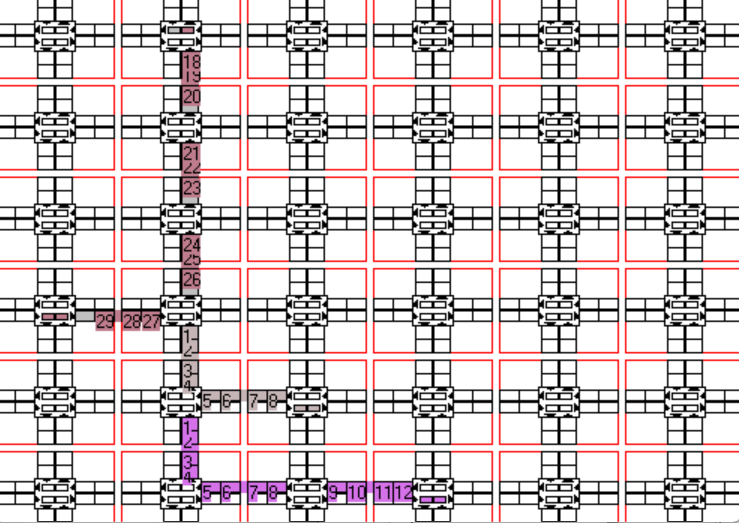
\includegraphics[width=\linewidth]{figs/congestion-simured.png}
    \caption{Encaminamiento determinista}
    %\label{fig:initial-bufferless}
  \end{subfigure}
  \hspace{0.25cm}
  \begin{subfigure}{0.48\textwidth}
    %\centering
    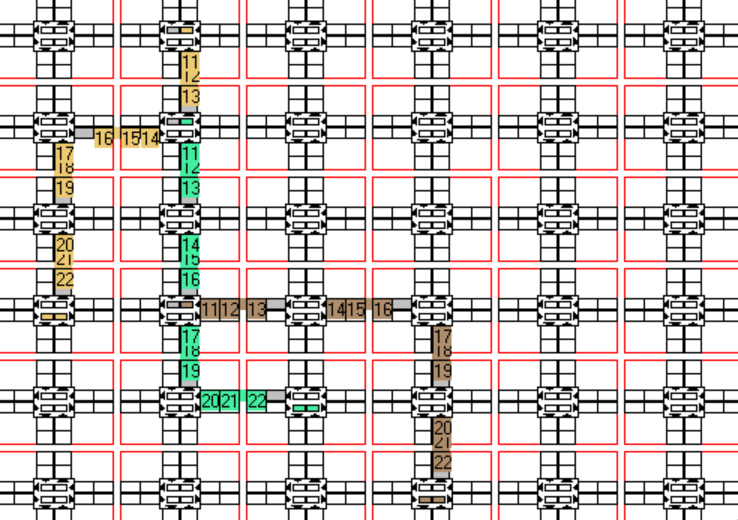
\includegraphics[width=\linewidth]{figs/adaptativo-simured.png}
    \caption{Encaminamiento adaptativo}
    %\label{fig:initial-bufferless}
  \end{subfigure}
  
  \vspace{1cm} % Add some vertical space
  
  \begin{subfigure}{0.48\textwidth}
    %\centering
    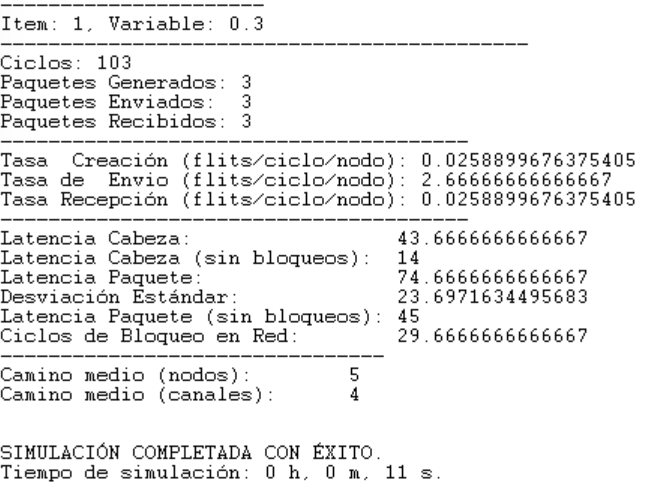
\includegraphics[width=\linewidth]{figs/determinista-estadisticas.png}
    \caption{Estadísticas encaminamiento determinista}
    %\label{fig:dropping}
  \end{subfigure}
  \hspace{0.25cm}
  \begin{subfigure}{0.48\textwidth}
    %\centering
    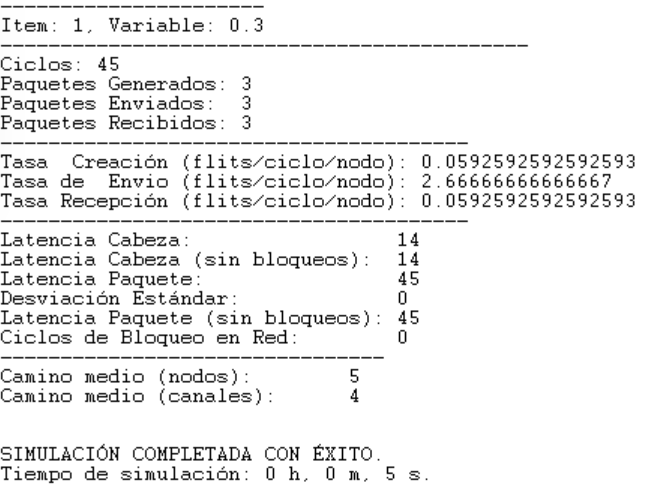
\includegraphics[width=\linewidth]{figs/adaptativo-estadisticas.png}
    \caption{Estadísticas encaminamiento adaptativo}
    %\label{fig:misrouting}
  \end{subfigure}
  \caption{Encaminamiento determinista vs adaptativo}
  \label{fig:detvsadap}
\end{figure}

    \item [\textbf{b)}] \textbf{Para comprobar las diferencias de una forma más clara entre los dos tipos de encaminamiento (en este caso determinista y el adaptativo de Duato), se realizará una evaluación más completa.}

    \textbf{Consistirá en obtener la latencia para diferentes tasas de inyección y comparar mediante las correspondientes gráficas los resultados para ambos algoritmos de encaminamiento. Un número recomendable de paquetes son $20000$ descartando, de cara a los resultados, del 5 al 10\% de los iniciales. Para este apartado utilizar la opción de guardar estadísticas en un fichero e ir acumulando los resultados en una misma gráfica para poder realizar las oportunas comparativas.}

    \item[\textbf{c)}] \textbf{Finalmente realizar una comparativa con diferente número de canales virtuales y justificar adecuadamente los resultados obtenidos.} 
    
\end{itemize}